\documentclass[../report_polarFIR.tex]{subfiles}
\begin{document}
\chapter{Cartesian \ac{FIR} Filter}

The FIR filter is implemented in Vitis HLS, using equations shown in section \ref{FIRtheory} to compute the 1-D convolution. The filter inputs have been specified on a range of $[-50, 50]$, which includes the filter coefficients. The computation of a convolution is rather simple, taking into account the fact that we have complex numbers to multiply (the filter weights, and the raw data to be processed). Generically, for complex vectors
\begin{equation}
	a = \alpha + j\beta
\end{equation}
and 
\begin{equation}
	b = \rho + j\delta
\end{equation}
we find their product $c = ab$ equivalent to
\begin{equation}
	c = (\alpha\rho - \beta\delta) + j(\alpha\delta+\beta\rho)
\end{equation}

This can be quickly translated into a processing algorithm shown below in Listing \ref{lst:FIRconv}.
\begin{quote}
\begin{singlespace}
    \lstinputlisting[breaklines=true,
     label={lst:FIRconv},
      caption={Convolution algorithm},
       style=c-style,
        language=C++,
         firstnumber=139,
          linerange={139-145}]{../source/complexFIR.cpp}
\end{singlespace}
\end{quote}

This algorithm is then instantiated across the whole dataset with the following function behavior:

\begin{quote}
\begin{singlespace}
    \lstinputlisting[breaklines=true,
     label={lst:FIRconv},
      caption={Filter pass control},
       style=c-style,
        language=C++,
         firstnumber=77,
          linerange={77-91}]{../source/complexFIR.cpp}
\end{singlespace}
\end{quote}


\section{Performance of the algorithm}
The performance of the algorithm can be broadly categorized into two major components:

\begin{quote}
\begin{description}
	\item [Latency] The computational time (clock cycles) required to process a valid result for a given input dataset.
	\item [Utilization] The amount of resources required to compute the result at a certain latency.
\end{description}
\end{quote}

Both of these metrics provide a general assessment of a given algorithm's performance. A high-efficiency algorithm minimizes utilization, and a high-performance algorithm minimizes latency. The combination of these two results in an ideally performing algorithm.

\subsubsection{Latency}
As emphasized in the introduction, the performance of the algorithm is a critical factor in its overall usability as a signal processor. One such metric of performance for the FIR filter is the computational latency necessary to compute a filter pass. We can estimate the optimized algorithm's latency prior to optimization with some optimizations:
\begin{enumerate}
	\item Element access (read/write) takes 1 cycle
	\item Addition takes 2 cycles
	\item Multiplication takes 4 cycles
\end{enumerate}
If we consider the filter pass shown in Listing \ref{lst:FIRconv}, it is possible to compute the number of cycles $Q$. $Q$ can be defined as 
\begin{equation}
	Q = X_i + A_i + M_i
\end{equation}
where $X_i$, $A_i$, $M_i$ are defined as 
\begin{equation}
	X_i = \sum_{i=0}^{numTaps} 1 = numTaps
\end{equation}
\begin{equation}
	A_i = \sum_{i=0}^{numTaps} 2 = 2 * numTaps
\end{equation}
\begin{equation}
	M_i = \sum_{i=0}^{numTaps} 4 = 4 * numTaps
\end{equation}
and subsequently 
\begin{equation}\label{FIRlatency}
	Q = (1 + 2 + 4)numTaps = 7 * numTaps
\end{equation}
 
 Assuming a filter size of $numTaps = 25$, we determine the latency to be approximately $Q$ = 175 cycles. This is, of course, just a single pass of the filter on a single datapoint, so multiple datapoints takes many more cycles. This has significant impact on the performance of the processing chain, and drastically increases system latency for a valid result. We synthesize an un-optimized filter using standard \codeword{int} datatypes within the system. The utilizations results below in Figure \ref{fig:unoptimizedFIRutil}. 
 
 \begin{figure}[h!]
 	\begin{center}
 		\fboxsep=0mm
 		\fbox{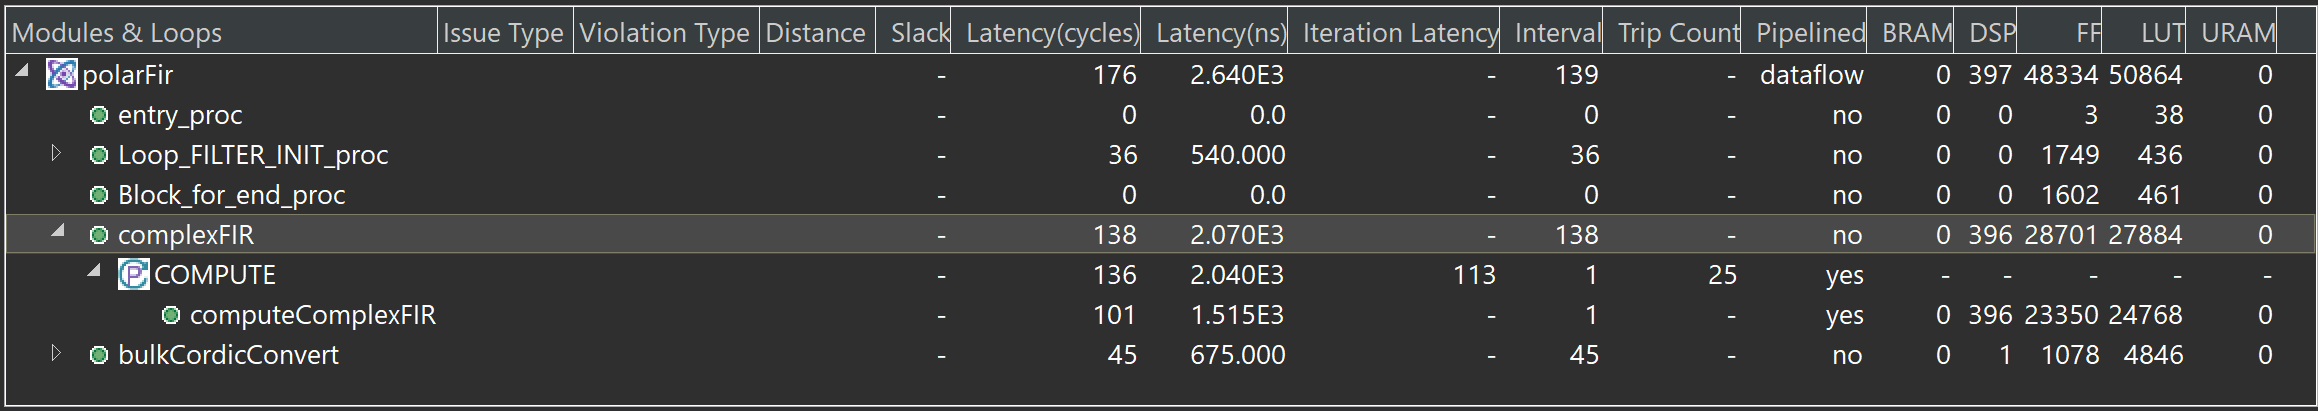
\includegraphics[width=\textwidth]{FIR/unoptimizedUtilReport.png}}
 		\caption{Un-optimized utilization report}
 		\label{fig:unoptimizedFIRutil}
 	\end{center}
 \end{figure}
 \FloatBarrier
 
 Note the high number of LUTs, FF, and DSPs necessary to run the design. The incredibly high utilization for the system has two problems. 1.) The design cannot be synthesized on the desired hardware target, and that chipset does not have enough resources. 2.) If enough hardware were available, the latency of over 130 cycles for the dataset is unacceptable for a realtime high performance system.
 
 \section{Optimization}
 To improve the performance of this algorithm, we leverage the \codeword{#pragma HLS} collection of compiler directives. These directives suggests to the compiler that it should rewrite or restructure the compiled result to improve the performance of the algorithm.
 
 \subsection{Unrolling}
Perhaps one of the most basic operations employed in the HLS environment is loop unrolling. Loop unrolling exploits parallelism on the device, and is commonly paired with \codeword{for} loop bodies. The behavior of the process effectively duplicates copies of the arguments inside of the loop, and reduces the iteration depth of the loop itself. This optimization is applied below in Listing \ref{lst:FIRunroll}.

\begin{quote}
\begin{singlespace}
    \lstinputlisting[breaklines=true,
     label={lst:FIRunroll},
     caption={Filter coefficient initialization},
     style=c-style,
     numbers=left,
     language=C++,
     firstnumber=54,
     linerange={54-59}]{../source/complexFIR.cpp}
\end{singlespace}
\end{quote}

\codeword{#pragma HLS UNROLL} in line 56 (Listing \ref{lst:FIRunroll}) completely unrolls the loop by a factor of \codeword{FILTER_SIZE} (which in this design is 25 taps), and as such reduces the computational latency to 1 cycle. This drastically reduces the computational latency required to calculate the result, and allows the core of the algorithm to start more quickly.

Another area this optimization is used is in the shift register within a computation of a filter pass itself. The shift register allows the system to exploit pipelined behavior, and allows data to be accessed in parallel. This is shown below in Listing \ref{lst:pipelineDelay}.


\begin{quote}
\begin{singlespace}
    \lstinputlisting[breaklines=true,
     label={lst:pipelineDelay},
     caption={Shift register},
     style=c-style,
     numbers=left,
     language=C++,
     firstnumber=123,
     linerange={123-136}]{../source/complexFIR.cpp}
\end{singlespace}
\end{quote}


\subsection{Pipelining}

While the ability to unroll a loop is useful, the parallelism exploited by unrolling a loop requires more discrete hardware. Resources like DSPs on an FPGA are incredibly precious, and as such it is important to ensure they are used to their maximum potential.

A commonplace method to increase throughput of a design in general is to pipeline the computational chain. This behavior is seen in nearly every modern-day processor, and enables high average resource utilization across the whole system. Of course, this also requires the system to be designed in such a manner conducive to pipeline architecture.

In the case of the FIR filter, it is possible to pipeline the design to achieve near-single-cycle latency. This is accomplished via the shift register implemented in Listing \ref{lst:pipelineDelay}, and the usage of \codeword{#pragma HLS PIPELINE}. 

It should be noted that the ability for a design to be pipelined also depends on parallel memory element access, and later sections will discuss this in greater detail.

\codeword{#pragma HLS PIPELINE} effectively converts loops that are a deterministic length at compile time into a pipelined design. At compile time, this precompiler directive attempts to achieve an iteration interval of 1 (\codeword{II = 1}), if this is not possible, it attempts to find the shortest-possible iteration interval that successfully pipelines the design. 

For example, consider the filter pass:


\begin{quote}
\begin{singlespace}
    \lstinputlisting[breaklines=true,
     label={lst:FIRconv},
      caption={Convolution algorithm},
       style=c-style,
        language=C++,
         firstnumber=139,
          linerange={139-145}]{../source/complexFIR.cpp}
\end{singlespace}
\end{quote}

Without the precompiler directive \codeword{#pragma HLS PIPELINE} on line 142, this loop takes a large amount of time to compute. This amount is estimated in equation \ref{FIRlatency}. 

Upon re-synthesis of the design with the precompiler directive the loop's performance is improved dramatically, reducing the number of cycles necessary to compute a result to an iteration interval of 1 (\codeword{II = 1}). This is a dramatic improvement in comparison to the old design. Additionally, the efficiency of the design also ensures that resources allocated for that element of the processing chain are at a maximal utilization.

\subsection{Dataset manipulation}

Perhaps not exactly ''optimization``, dataset manipulation in the HLS environment is the second step (first is a good design) to structure code for optimization. Standard C/C++ languages transfer data between functions as linear allocation. Consider an array \texttt{X} which contains $N$ elements. The array is typically organized in memory as a sequential set of data:
\begin{figure}[h!]
\begin{center}
\begin{bytefield}{16}
\bitbox{4}{\texttt{X[0]}} \bitbox{4}{\texttt{X[1]}} \bitbox{4}{$\dots$}\bitbox{4}{\texttt{X[N]}}
\end{bytefield}

\caption{Standard array format}
\end{center}
\end{figure}

This structure works rather well for traditional linear programs, as it allows efficient allocation of the program memory. However, parallel access of the array is not possible, as the same chunk of memory would be referenced by multiple scheduled calls. This fails to access at the best, and crashes the system at the very worst. To mitigate this problem, it is possible to reshape the array into a format conducive to parallel access. 

The usage of \codeword{#pragma HLS ARRAY_PARTITION} in the HLS environment provides the ability to transpose any given array with a variety of configurable parameters. A trivial method is to partition the array completely, resultant in the following data structure:

\begin{figure}[h!]
\begin{center}
\begin{bytefield}{4}
\bitbox{4}{\texttt{X[0]}}\\
\bitbox{4}{\texttt{X[1]}}\\
\bitbox{4}{$\dots$}\\
\bitbox{4}{\texttt{X[N]}}\\
\end{bytefield}
\caption{Partitioned array (complete)}
\label{fig:arrayPartComplete}
\end{center}
\end{figure}

The structure shown in Figure \ref{fig:arrayPartComplete} utilizes complete partioning. This means that each element can be accessed in parallel at any time, without read/write conflicts. However, this also increases the number of storage elements necessary to allow this transposition. In situations where a complete partition is not viable or computationally necessary, it is possible to partition the array with a varying factor. For example, partitioning the array X with a factor of 3 achieves the following data structure:

\begin{figure}[h!]
\begin{center}
\begin{bytefield}{12}
\bitbox{4}{\texttt{X[0]}} \bitbox{4}{\texttt{X[1]}} \bitbox{4}{\texttt{X[2]}}\\
\bitbox{4}{$\dots$} \bitbox{4}{$\dots$} \bitbox{4}{$\dots$}\\
\bitbox{4}{$\dots$} \bitbox{4}{$\dots$} \bitbox{4}{$\dots$}\\
\bitbox{4}{\texttt{X[N-3]}} \bitbox{4}{\texttt{X[N-1]}} \bitbox{4}{\texttt{X[N]}}\\
\end{bytefield}
\caption{Partitioned array (factor of 3)}
\label{fig:arrayPartComplete}
\end{center}
\end{figure}
\FloatBarrier

This allows array elements to be accessed in multiples of three. To utilize the array in this manner, a factor of 3 should be present in the design when unrolling or pipelining. The advantages of higher-factor partitioning reduces the discrete hardware necessary to store an element of data, at the potential cost of increased design latency.

Despite the advantages of higher-factor partitioning, the simplicity of the FIR filter, and its small number of taps, is conducive to complete array partitions on data in the system. For example, Listing \ref{lst:FIRarraypart} shows how the pipeline shift registers are partitioned.


\begin{quote}
\begin{singlespace}
    \lstinputlisting[breaklines=true,
     label={lst:FIRarraypart},
      caption={Convolution algorithm},
       style=c-style,
        language=C++,
         firstnumber=113,
          linerange={113-117}]{../source/complexFIR.cpp}
\end{singlespace}
\end{quote}

\subsection{Datatypes}\label{FIRdata}

An interesting area for optimization in an HLS environment is the usage of arbitrary-width datatypes. In a traditional C/C++ environment, the amount of memory available usually provides no reason to use custom types. Additionally, because a traditional C program runs on a fixed-width data structure, anything other than 8/32/64/128-bit architecture is inefficient and often unnecessary.

The difference between a traditional C program and a HLS product is that HLS products are synthesized into a product for deployment on an FPGA. Because FPGAs have fully reprogramable logic/DSP slices, it is possible to use data widths of any kind in a design.

That being said, there are a few technical constraints or considerations to be made in choosing the size of a given datatype. The DSPs on an FPGA are limited in their input data sizes. In the case of Xilinx's DSP48 on the Zynq-7000 series FPGA, it is possible to multiply a 25 and 18 bit number on a single DSP slice. Therefore, operations that exceed 25x18 bits will leverage multiple DSPs to compute the result. Standard \codeword{int} and \codeword{float} datatypes require 32 bits to calculate, and therefore would require at least 3 DSP slices to compute.

Another consideration is the input/output range of the design, in addition to signage or required precision. It is possible to compute the number of bits required for any given number using the equation

\begin{equation}\label{widthEQ}
	K = \lceil log_2{|x|} \rceil
\end{equation}

where $K$ is the computed number of bits, and $x$ is the number in question. If $x$ is a decimal number, it's necessary to shift the number's decimal to the end of the decimal for the calculation. For example the number $x = 9000$ requires 14 bits, and the number $x = 10.0025$ requires 17 bits.

We can also use this equation to determine the number of bits necessary to handle data in/out of the FIR filter. Consider a worst-case scenario for the input dataset $\overline X$ and filter coefficients $w_i$ of
\begin{equation*}
	\overline X = [50 + j50, 50 + j50,...,50+j50]^T
\end{equation*}
and
\begin{equation*}
	w_i = [50 + j50, 50 + j50,...,50+j50]^T
\end{equation*}
where the input data size is arbitrary, but the span of $w_i$ is fixed to 25 taps. Applying the FIR filter to a datapoint, we find the output of the filter $\overline Y$ to be
\begin{equation*}
	\overline Y_{max} = 2 * 50^2 * 25 = 125,000 
\end{equation*}

as a worst-case maximum. Of course, this also works for a worst-case minimum, which generates  $\overline Y_{min} = -125,000$. These results are applied to equation \ref{widthEQ}, determining the results of $K_{in}$ for the inputs, and $K_{out}$ for the output bitwidth required:
\begin{equation}
	K_{in} = \lceil log_{2}{|50|} \rceil = 6
\end{equation}
\begin{equation}
	K_{out} = \lceil log_{2}{|125000|} \rceil = 17
\end{equation}

These results are applied to arbitrary precision datatypes in the design, and contribute significantly to the reduction of resource utilization in the design.

\subsubsection{Arbitrary precision}

The HLS environment offers arbitrary precision datatypes for signed or unsigned integers, and fixed-point decimals. When leveraged properly, the usage of these data types dramatically increases design performance. 

To use this functionality, we access functions in the \codeword{ap_int.h} and \codeword{ap_fixed} libraries. The results obtained for $K_{in}$ and $K_{out}$ translate into the following design datatypes seen in Listing \ref{datatypeCode}


\begin{quote}
\begin{singlespace}
    \lstinputlisting[breaklines=true,
     label={datatypeCode},
      caption={System datatypes},
       style=c-style,
        language=C++,
         firstnumber=20,
          linerange={20-23}]{../source/datatypes.h}
\end{singlespace}
\end{quote}

Utilization of these new datatypes as \codeword{typedef}s is not incredibly complex, but does require consultation of HLS documentation for utilization functions. Conversion between datatypes, or printing results to the console requires specific syntax.

\subsection{Optimization results}

Optimization performed to the algorithm has dramatically reduced the design's latency and utilization. This result was only possible after the careful insertion of precompiler directives, and one's ability to structure the algorithm in a manner conducive to parallel processing. It should be noted that there are still design limitations that exist. Namely, the ability to load data input into the filter itself. Because the top-level architecture requires variable input lengths, there's nothing that can be done to improve element access, as those elements are passed as a pointer of unknown size (i.e. \codeword{int *foo} instead of \codeword{int foo[4]}).

Below in Figure \ref{optimizedFIRutil} is the utilization report generated from HLS upon synthesis of the computational system. 

 \begin{figure}[h!]
 	\begin{center}
 		\fboxsep=0mm
 		\fbox{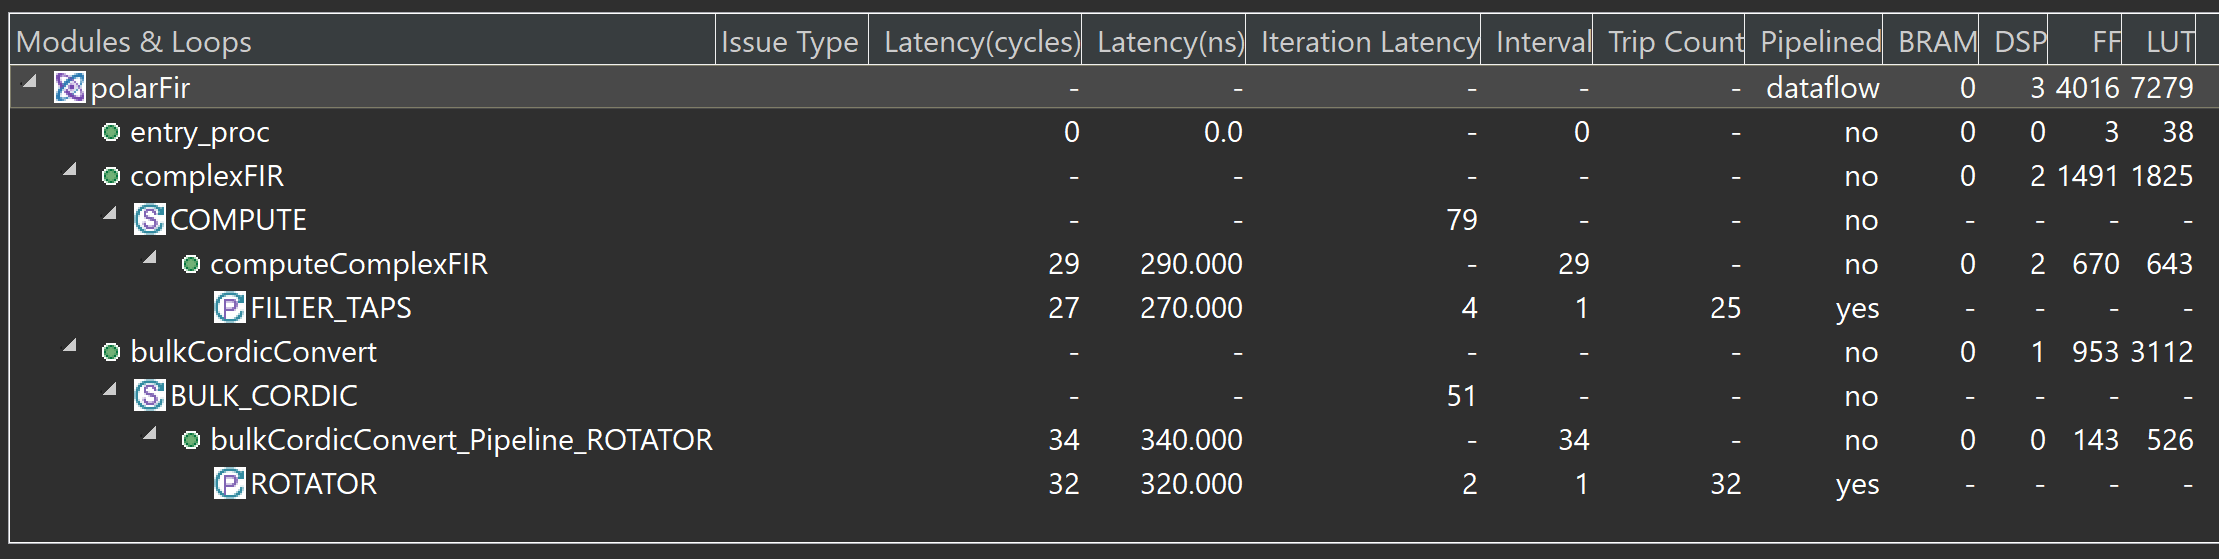
\includegraphics[width=\textwidth]{media/optimizedUtilReport.png}}
 		\caption{Optimized utilization report}
 		\label{optimizedFIRutil}
 	\end{center}
 \end{figure}
 \FloatBarrier
 
 Analysis of this report, along with the un-optimized report shown in Table \ref{fig:unoptimizedFIRutil}, shows the following changes in resource utilization for the FIR filter, with amazing results.
 
 
\begin{table}[h!]
    \centering
    
    \begin{tabular}{|l|l|l|l|}
        \hline
		\textbf{Resource type} & \textbf{Before} & \textbf{After} & \textbf{\% Change} \\
		\hline \hline
		DSP & 396 & 2 & -99.5\% \\
		\hline
		Flip-flops & 28701 & 670 & -97.6\% \\
		\hline
		Lookup tables & 27884 & 643 & -97.7\% \\
	\hline
		
    \end{tabular}
    \label{FIRresourceComparison}
    \caption{FIR filter utilization before and after optimization}
\end{table}
\FloatBarrier

The original design was so inefficient that the FIR in combination with the CORDIC was impossible to implement on the Zynq chipset in use. Optimization of the program structure and datatypes has dramatically increased the design's performance.

Another area of optimization for the design is latency. Perhaps not as dramatic a change as the utilization, there was still a substantial increase in the design performance. These results are summarized in Table 
 
 \begin{table}[h!]
    \centering
    
    \begin{tabular}{|l|l|l|l|}
        \hline
		\textbf{Latency cycles} & \textbf{Before} & \textbf{After} & \textbf{\% Change} \\
		\hline \hline
		Total & 136 & 27 & -80.2\% \\
		\hline
		Iteration latency & 113 & 79 & -30.1\% \\
	\hline
		
    \end{tabular}
    \label{FIRresourceComparison}
    \caption{FIR filter latency before and after optimization}
\end{table}
\FloatBarrier

Again, this result is well-recieved for the design. The results suggest that the design has been highly optimized for computational latency and resource utilization. This design would be adventageous to integrate into a more complete processing chain, as it uses a small amount of resources continually and computes a result with minimal latency.


\end{document}